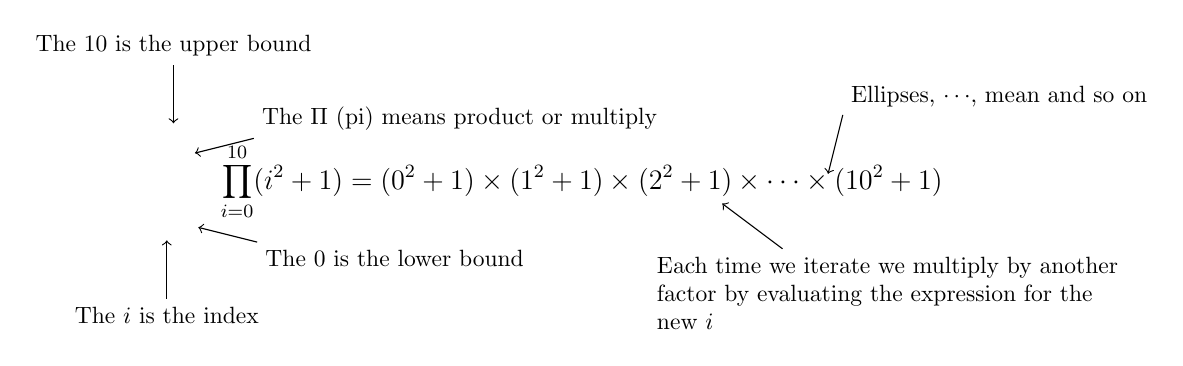
\begin{tikzpicture}[scale=0.85,transform shape]
% Main Expression
    \node[font=\large] at (0,0) {\(\displaystyle\prod_{i=0}^{10} (i^2+1) = (0^2+1) \times (1^2+1) \times (2^2+1) \times \cdots \times (10^2+1)\)};
% Lables
    \draw[<-,shorten <= 3pt] (3.65,0) -- +(0.25,1) node[anchor=south west] {Ellipses, \(\cdots\), mean and so on};
    \draw[<-,shorten <= 3pt] (-5.9,0.4) -- +(1,0.25) node[anchor=south west] {The \(\Pi\) (pi) means product or multiply};
    \draw[<-,shorten <= 3pt] (-6.1,0.75) -- +(0,1) node[anchor=south] {The \(10\) is the upper bound};
    \draw[<-,shorten <= 3pt] (-6.2,-0.75) -- +(0,-1) node[anchor=north] {The \(i\) is the index};
    \draw[<-,shorten <= 3pt] (-5.85,-0.65) -- +(1,-0.25) node[anchor=north west] {The \(0\) is the lower bound};
    \draw[<-,shorten <= 3pt] (2,-0.25) -- +(1,-0.75) node[anchor=north west,text width=7cm,xshift=-2cm] {Each time we iterate we multiply by another factor by evaluating the expression for the new \(i\)};    
% Helper Grid
    % \draw[step=1] (-7,-1) grid (7,1);
    % \draw[step=0.5,dashed] (-7,-1) grid (7,1);
    % \node[anchor=north] at (0,-1) {0};
\end{tikzpicture}